%\section{Dizionario dati}
\section{Catalogo dati}

Una volta che CKAN � stato popolato di dataset si � realizzato il catalogo dei dataset presenti.
Per fare ci� � stato necessario recuperare le informazioni contenute nel database e quindi le tabelle prese in esame sono state \texttt{package}, \texttt{resource} e \texttt{resource\_group}. La loro struttura � mostrata in figura \ref{fig:DB-design}:

\begin{figure}[htbp]
   \centering
   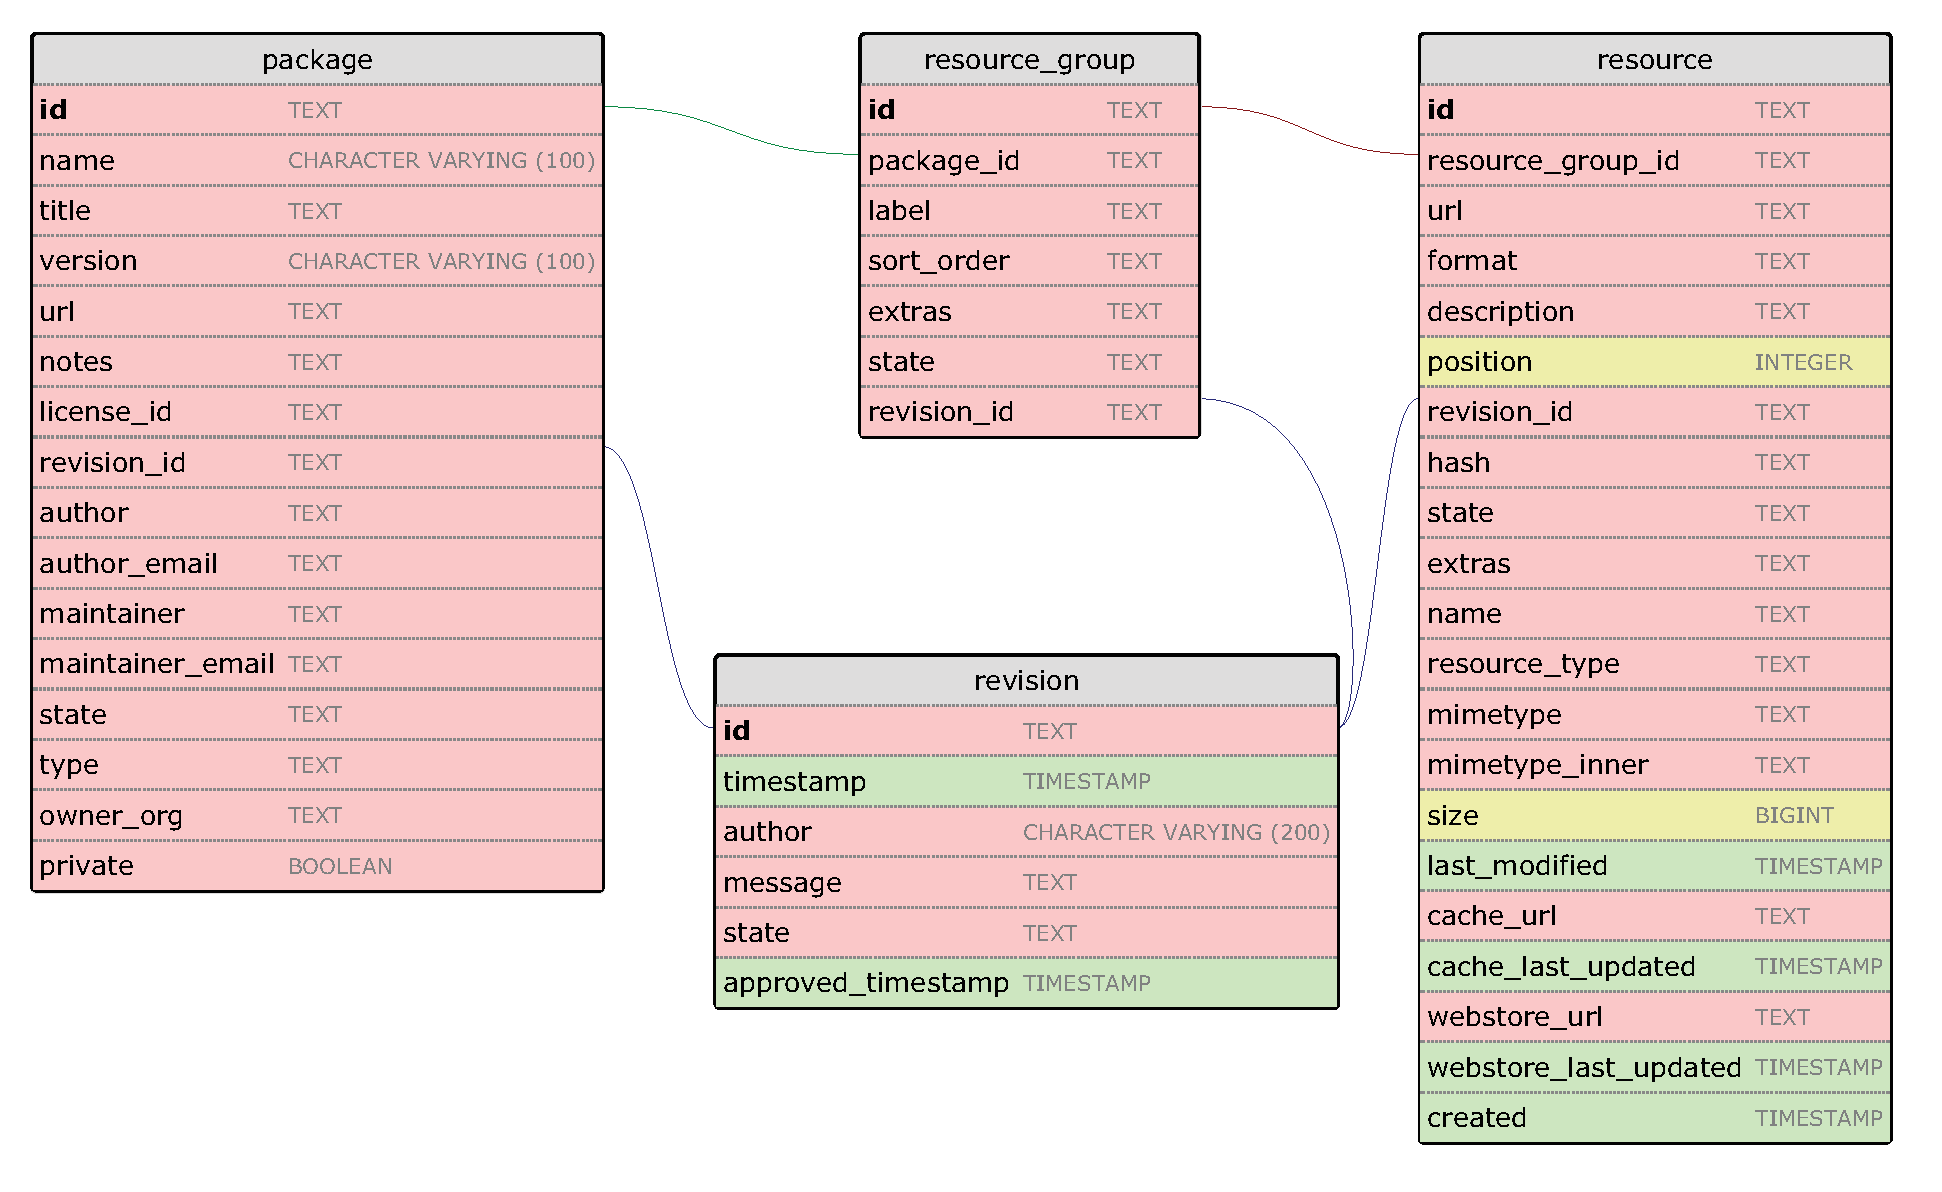
\includegraphics[scale=0.40]{img/DB-design2}
   \caption{Design DataBase}
   \label{fig:DB-design}
\end{figure}

Le informazioni sono presenti in tabelle differenti, ed � quindi stato necessario fare un JOIN tra le 3 tabelle e successivamente selezionare solo i campi di nostro interesse. Inoltre si sono tradotte le intestazioni delle colonne in italiano e si � creato un nuovo campo (link) concatenando l�url base della piattaforma con le informazioni presenti nel database.
%Per realizzare tutto ci� si � utilizzato la seguente query:\\
%{\indent{\footnotesize \verb$SELECT "name" AS "nome", "description" AS "descrizione", "url" AS "url",$}}\\
%{\indent{\footnotesize \verb$ "format" AS "formato", "last_modified" AS "ultima modifica",$}}\\
%{\indent{\footnotesize \verb$ "author" AS "autore", "author_email" AS "email autore",$}}\\
%{\indent{\footnotesize \verb$ "maintainer" AS "manutentore", "maintainer_email" AS "email manutentore",$}}\\
%{\indent{\footnotesize \verb$ CONCAT('http://localhost/dataset/',url_name,'/resource/',url_id) AS "link"$}}\\
%{\indent{\footnotesize \verb$FROM	($}}\\
%{\indent{\footnotesize \verb$ SELECT	"name", "description", "url", "format", "last_modified",$}}\\
%{\indent{\footnotesize \verb$   "resource_group_id", "package_id", resource.id AS "url_id"$}}\\
%{\indent{\footnotesize \verb$ FROM	"resource_group"$}}\\
%{\indent{\footnotesize \verb$ JOIN	"resource"$}}\\
%{\indent{\footnotesize \verb$ ON	resource_group.id=resource.resource_group_id$}}\\
%{\indent{\footnotesize \verb$ WHERE	"name"<>'datacatalog.csv'$}}\\
%{\indent{\footnotesize \verb$ ) AS "resource"$}}\\
%{\indent{\footnotesize \verb$JOIN	($}}\\
%{\indent{\footnotesize \verb$ SELECT	"id", "author", "author_email", "maintainer", "maintainer_email",$}}\\
%{\indent{\footnotesize \verb$  "name" AS "url_name"$}}\\
%{\indent{\footnotesize \verb$ FROM	"package") AS "package"$}}\\
%{\indent{\footnotesize \verb$ON	resource.package_id=package.id$}}\\
%{\indent{\footnotesize \verb$ORDER BY "last_modified" DESC;$}}\\

Ci� � stato realizzato attraverso una query, il cui risultato � stato esportato in un file in formato CSV (comma-separated values). Si � voluto salvare il file in una posizione che fosse poi recuperabile dal web server, di conseguenza si � scelto di salvarlo nella sua root. Ci� � possibile utilizzando il comando \textit{Copy} dopo aver acceduto al database PostgreSQL:\\

\shellcmd{sudo psql -h localhost -U ckanuser ckan\_default}
{\indent\indent{\footnotesize \verb$\Copy ($}}\\
\\
\centerline{\texttt{...QUERY...}}\\
\\
{\indent\indent{\footnotesize \verb$) To '/usr/lib/ckan/default/src/ckan/ckan/public/datacatalog.csv'$}}\\
{\indent\indent{\footnotesize \verb$With CSV HEADER$}}\\

  
Successivamente, per automatizzare il processo di creazione del catalogo ad ogni nuovo inserimento di un dataset in CKAN, sono stati creati una funzione ed un trigger.

Per fare ci� si accede a postreSQL e si assegnano i permessi di SuperUser all�utente utilizzato per creare il database:\\

\shellcmd{sudo -u postgres psql}
{\indent\indent{\footnotesize \texttt{\footnotesize\textcolor{NavyBlue}{=\#}} \verb#alter role ckanuser SUPERUSER;#}}\\

Ci� � necessario affinch� la funzione che andiamo a creare possa esportare il database all�esterno dell�ambiente.
Accediamo quindi al database e procediamo con la creazione di funzione e trigger:\\

\shellcmd{sudo psql -h localhost -U ckanuser ckan\_default}

La funzione non fa altro che eseguire l'esportazione della query in CSV nella posizione prestabilita:\\

{\indent{\footnotesize \verb#CREATE FUNCTION create_datacatalog ()#}}\\
{\indent{\footnotesize \verb#RETURNS trigger#}}\\
{\indent{\footnotesize \verb#AS $create_datacatalog$#}}\\
{\indent{\footnotesize \verb#BEGIN EXECUTE '#}}\\
{\indent{\footnotesize \verb#Copy (SELECT "name" AS "nome", "description" AS "descrizione", "url" AS#}}\\
{\indent{\footnotesize \verb# "url", "format" AS "formato", "last_modified" AS "ultima modifica",#}}\\
{\indent{\footnotesize \verb# "author" AS "autore", "author_email" AS "email autore", "maintainer"#}}\\
{\indent{\footnotesize \verb# AS "manutentore", "maintainer_email" AS "email manutentore" FROM (#}}\\
{\indent{\footnotesize \verb# SELECT "name", "description", "url", "format", "last_modified",#}}\\
{\indent{\footnotesize \verb# "resource_group_id", "package_id", resource.id AS "url_id"#}}\\
{\indent{\footnotesize \verb# FROM "resource_group" JOIN "resource"#}}\\
{\indent{\footnotesize \verb# ON resource_group.id=resource.resource_group_id) AS "resource"#}}\\
{\indent{\footnotesize \verb# JOIN (SELECT "id", "author", "author_email", "maintainer",#}}\\
{\indent{\footnotesize \verb# "maintainer_email", "name" AS "url_name" FROM "package") AS "package"#}}\\
{\indent{\footnotesize \verb# ON resource.package_id=package.id ORDER BY "last_modified" DESC)#}}\\
{\indent{\footnotesize \verb# To ''/usr/lib/ckan/default/src/ckan/ckan/public/datacatalog.csv''#}}\\
{\indent{\footnotesize \verb# With CSV HEADER;#}}\\
{\indent{\footnotesize \verb#';#}}\\
{\indent{\footnotesize \verb#RETURN NEW;#}}\\
{\indent{\footnotesize \verb#END;#}}\\
{\indent{\footnotesize \verb#$create_datacatalog$#}}\\
{\indent{\footnotesize \verb#LANGUAGE plpgsql;#}}\\
\\
Mentre invece il trigger si attiva ad ogni modifica della tabella \texttt{resource} e invoca la funzione:\\

{\indent{\footnotesize \verb#CREATE TRIGGER datacatalog_update#}}\\
{\indent{\footnotesize \verb#AFTER insert OR update#}}\\
{\indent{\footnotesize \verb#ON resource#}}\\
{\indent{\footnotesize \verb#FOR EACH ROW#}}\\
{\indent{\footnotesize \verb#EXECUTE PROCEDURE create_datacatalog();#}}\\
\\

Infine per rendere possibile la modifica del file \texttt{datacatalog.csv} da parte del web server si `e assegnato al file i permessi di scrittura all�utente \texttt{postgresql}:\\

\shellcmd{sudo touch /usr/lib/ckan/default/src/ckan/ckan/public/datacatalog.csv}
\shellcmd{sudo chmod 644 /usr/lib/ckan/default/src/ckan/ckan/public/datacatalog.csv}
\shellcmd{sudo chown postgres:postgres /usr/lib/ckan/default/src/ckan/ckan\\/public/datacatalog.csv}


\section{Dizionario dati}
Nelle intenzioni dello sviluppo della piattaforma si � cercato di aggiungere nel catalogo anche le informazioni sul tipo di dato contenuto in ogni singolo dataset. In pratica si voleva inserire un�ulteriore colonna nel catalogo contenente le intestazioni della tabella del dataset.
Purtroppo non si � trovata una soluzione per realizzare questa feature in quanto non si � trovato il modo di recuperare le informazioni presenti nei due differenti database che sono relazionati come mostrato in figura \ref{fig:DBs-ckan}:

\begin{figure}[htbp]
   \centering
   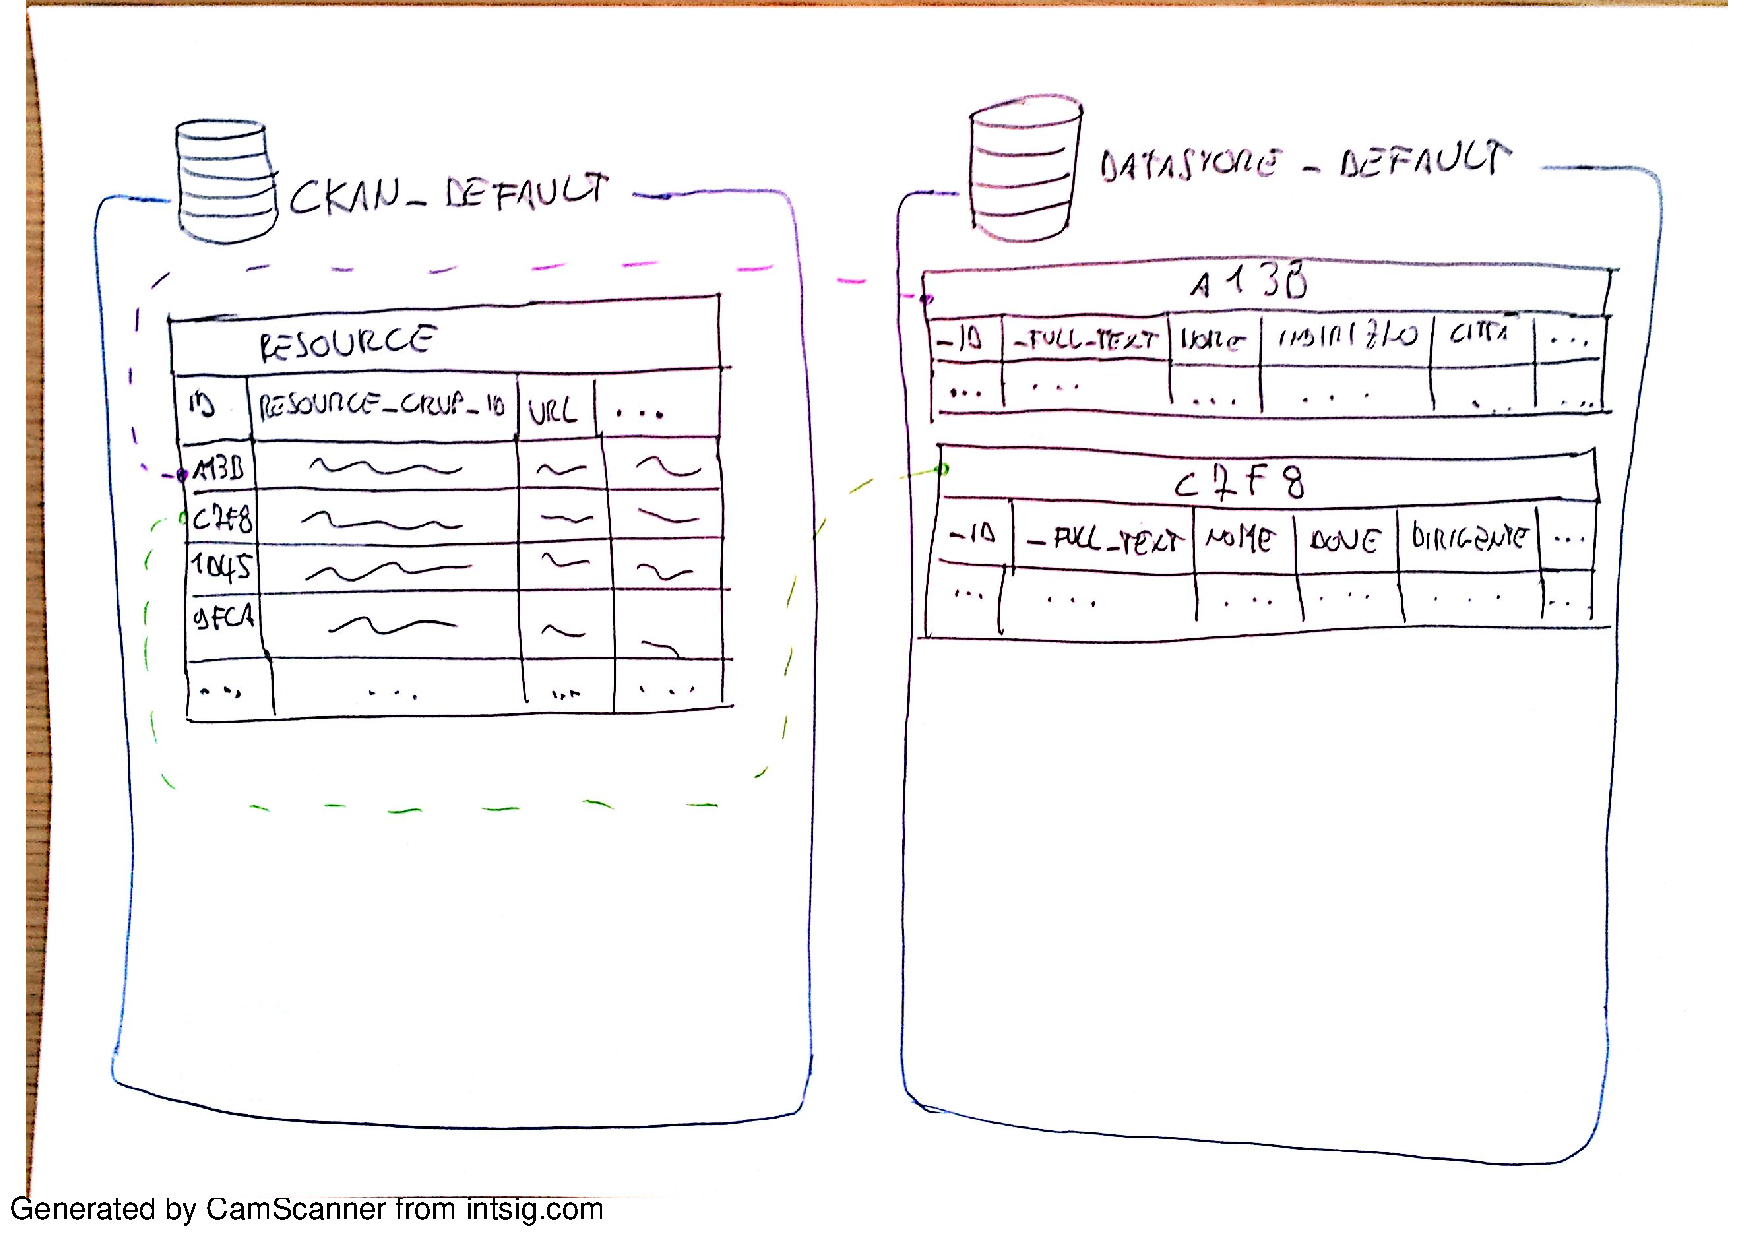
\includegraphics[scale=0.50,trim=1cm 7cm 0 3cm, clip=true]{img/DBs-ckan}
   \caption{relazione tra le tabelle dei DataBase utilizzati da CKAN}
   \label{fig:DBs-ckan}
\end{figure}

L�impossibilit� di recuperare l�intestazione delle tabelle del database \texttt{datastore\_default} una volta conosciuto il valore nel campo \texttt{id} dei singoli elementi presenti nella tabella \texttt{resource} del database \texttt{ckan\_default} non ha quindi al momento permesso la creazione del dizionario dati.